\chapter{Supplemental Figures}

\begin{figure}[h]
    \centering
    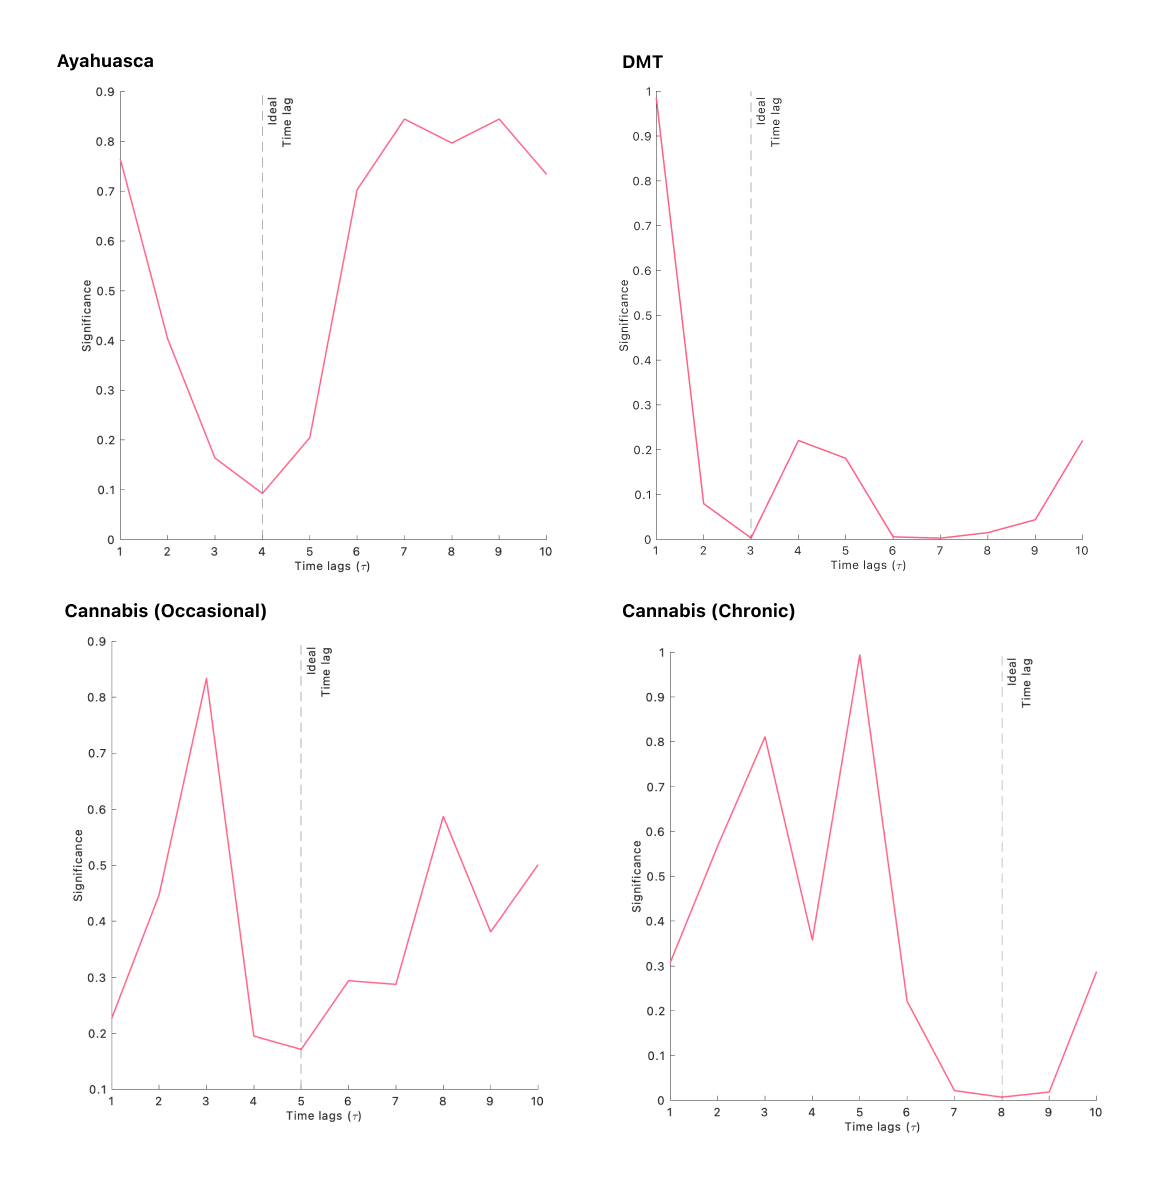
\includegraphics[width=\textwidth]{images/Appendix_ Tau Calculation.png}
    \caption{Evaluation of the ideal time-delay constant $\tau$ for each condition. Model-free irreversibility was calculated for Tau values 1 through 10 for each condition. For ayahuasca, occasional and chronic use of cannabis, a Wilcoxon rank-sum test was used to evaluate significance. The ideal Tau was determined as the most sensitive measure which best discriminates between baseline or placebo and drug conditions. For DMT, a mixed effects model was used in order to account for the pre-injection data as a covariate.}
    \label{fig:tau}
\end{figure}

\begin{figure}[h]
    \centering
    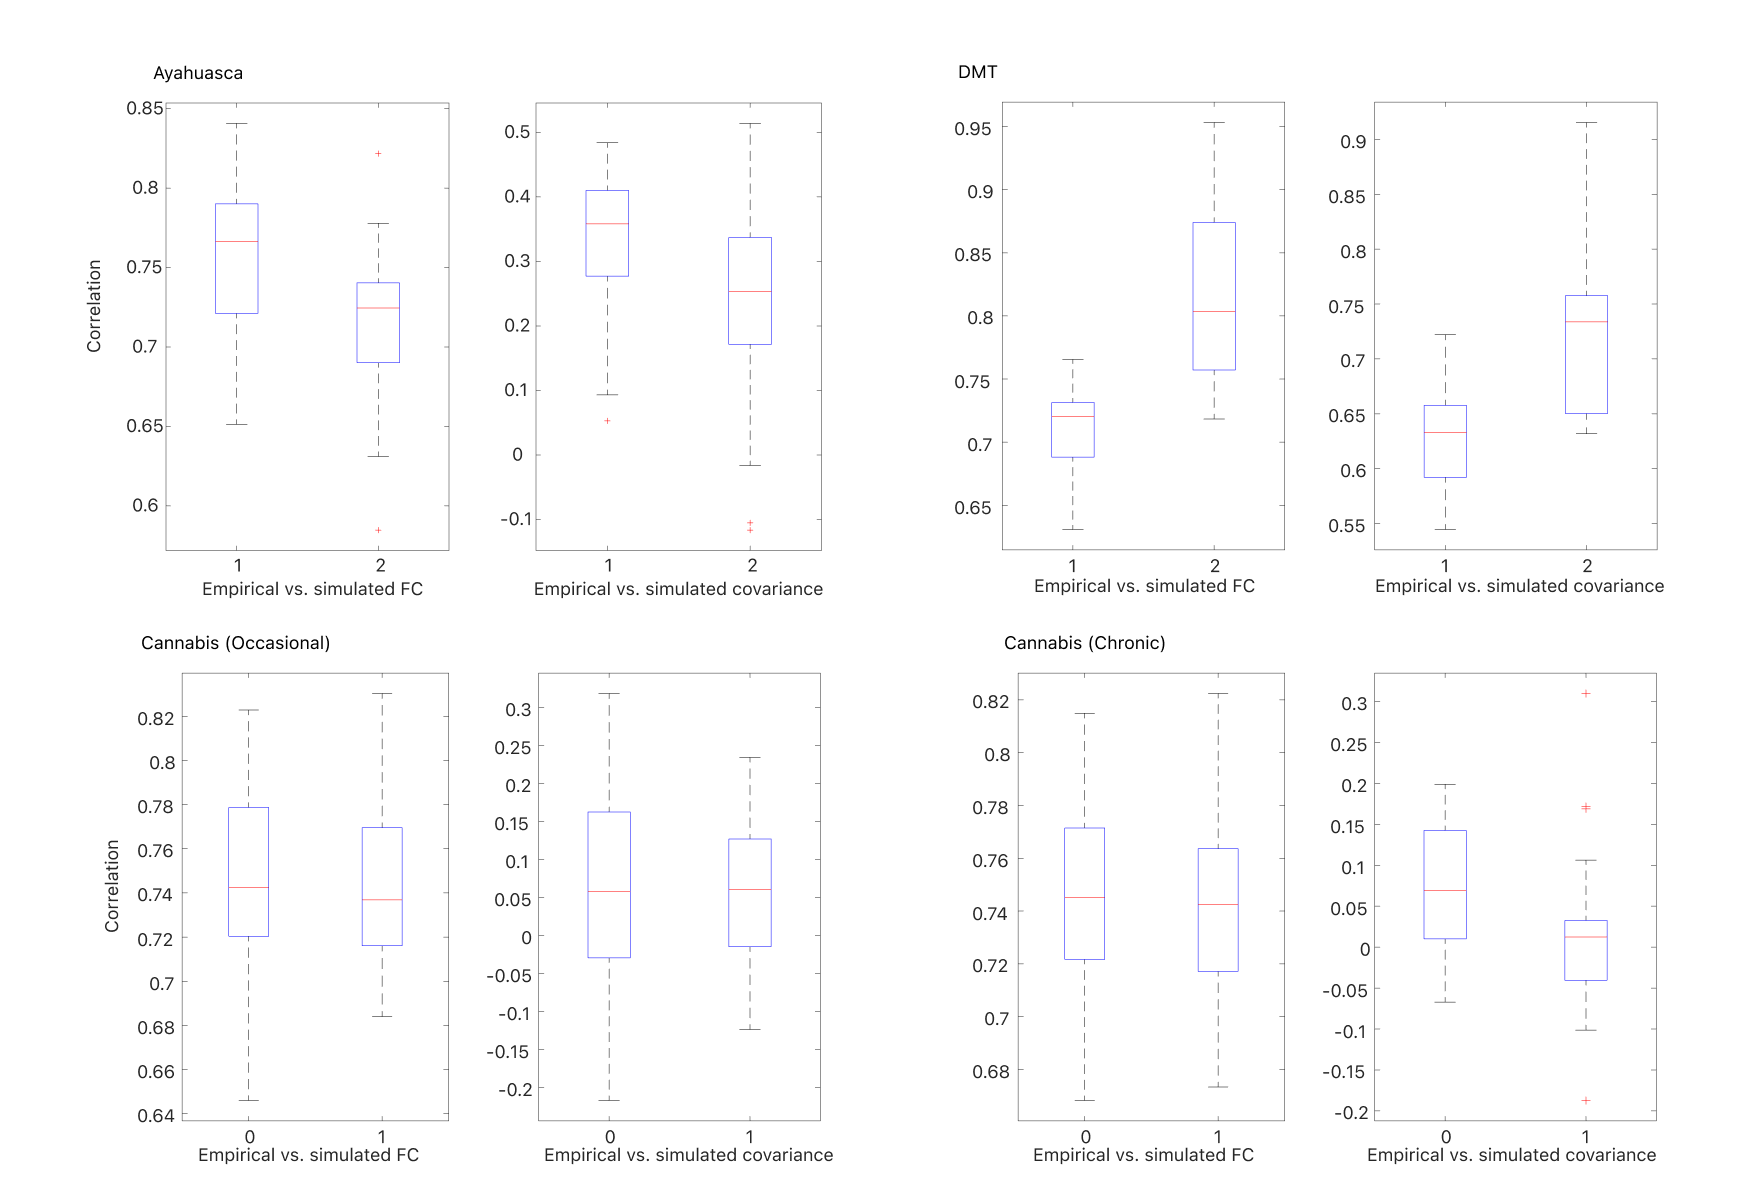
\includegraphics[width=\textwidth]{images/Appendix_ Fits.png}
    \caption{Correlations between empirical and simulated functional connectivity (left panel, each condition), and between empirical and simulated covariance of irreversibility matrices (right panel, each condition). "1" indicates baseline or placebo condition. "2" indicates drug condition.}
    \label{fig:fits}
\end{figure}

\begin{figure}
    \centering
    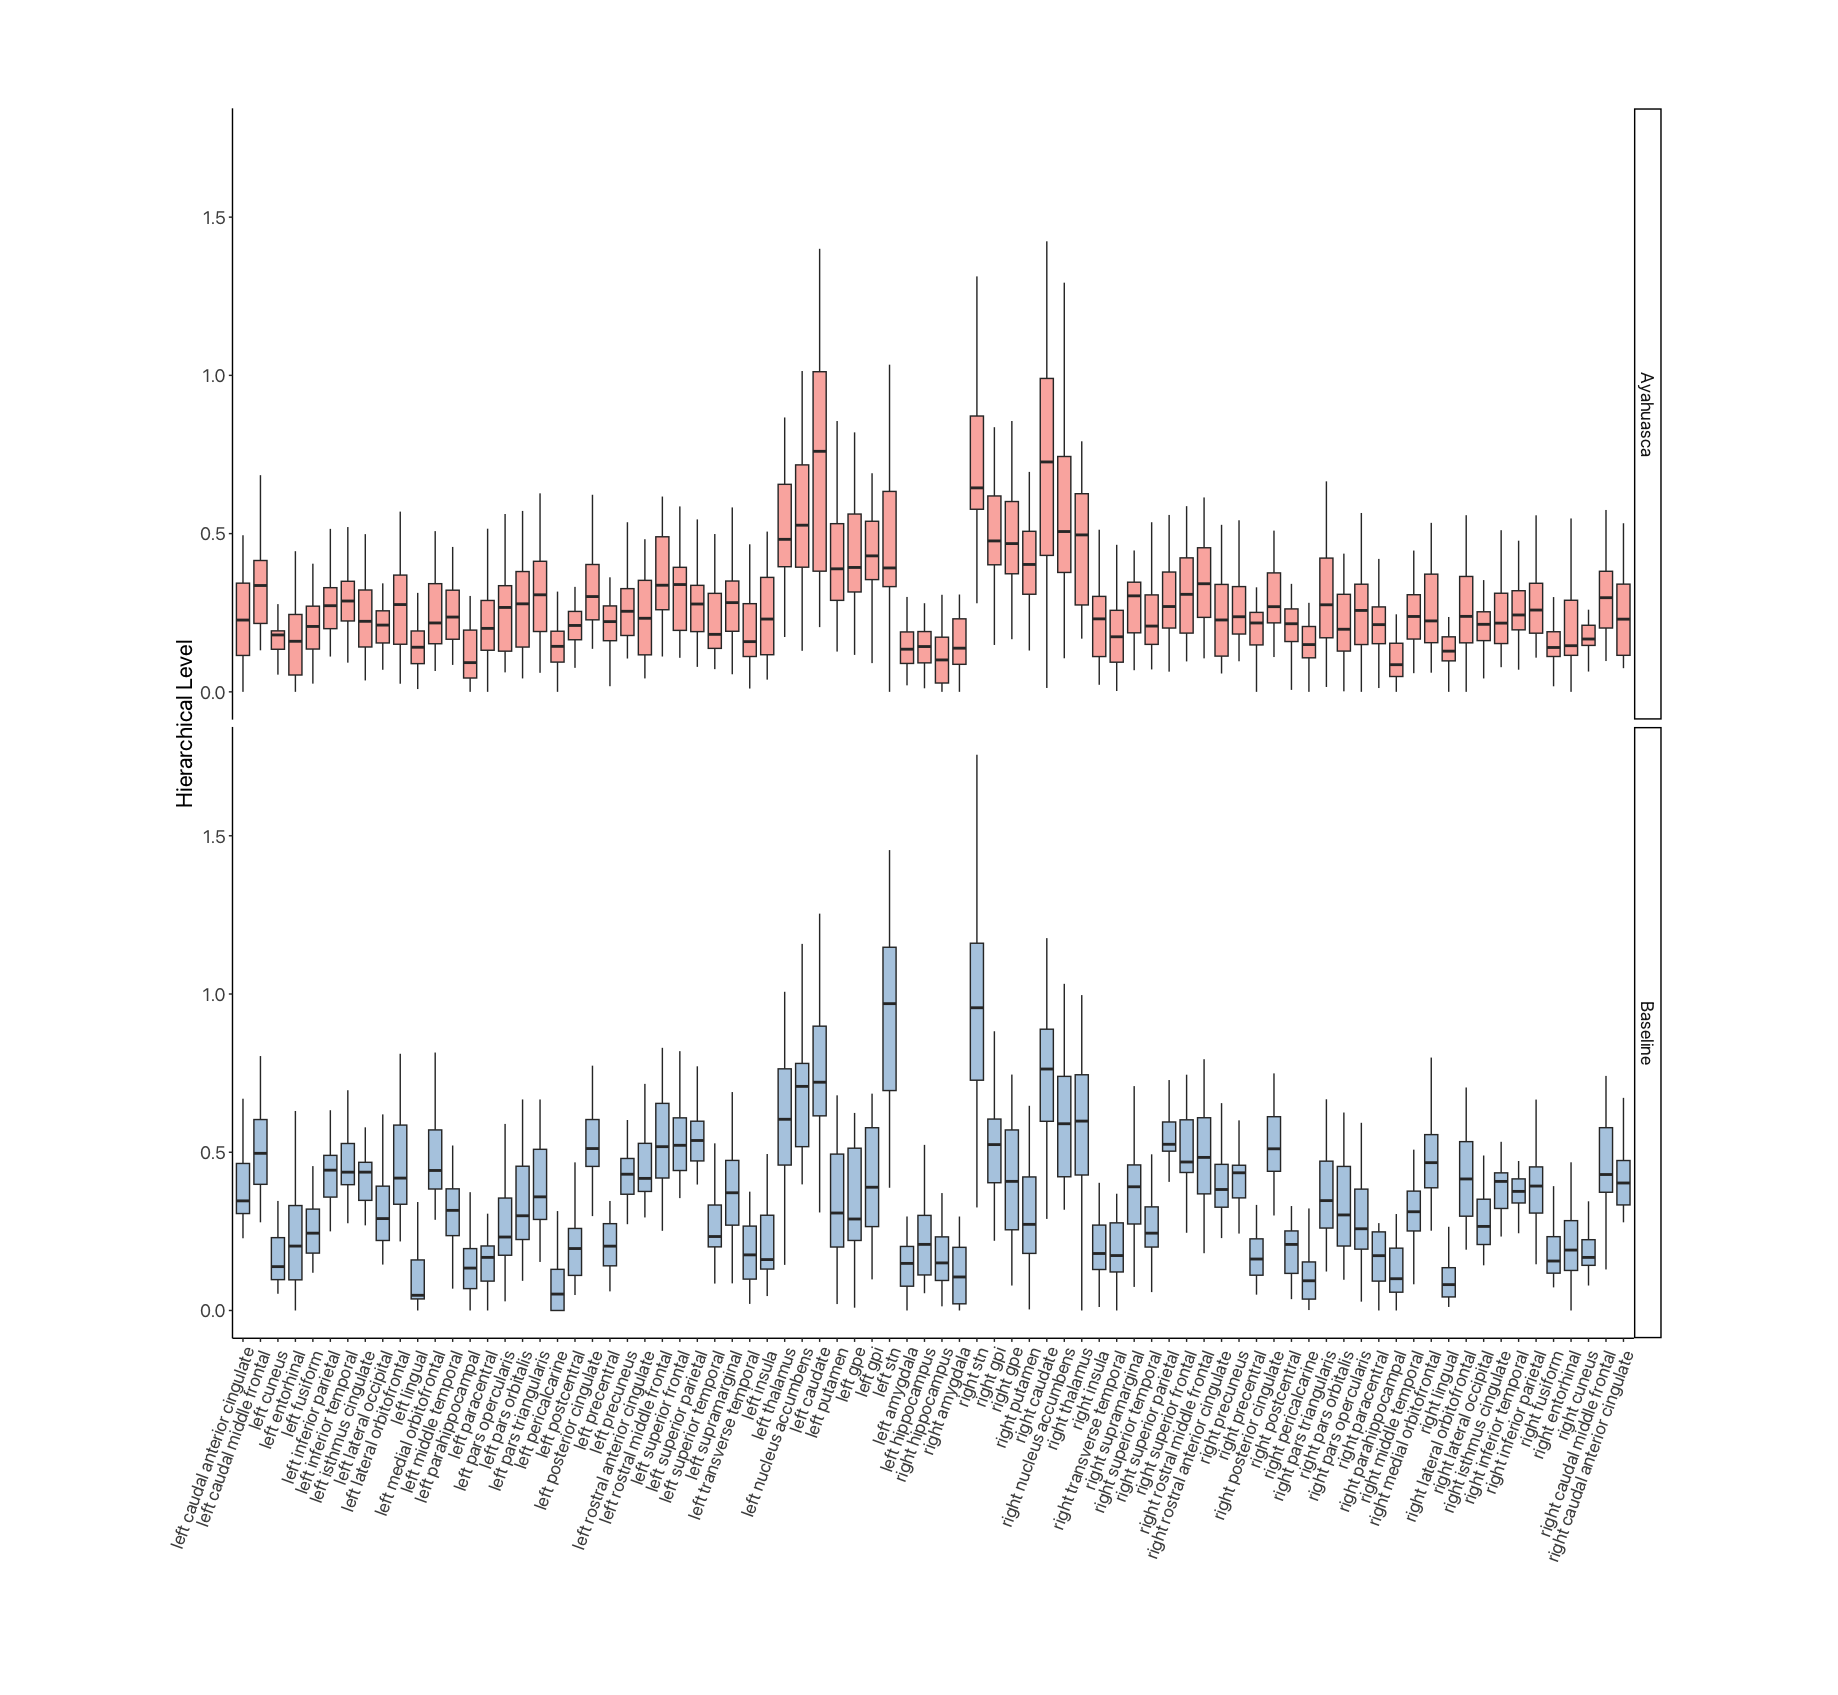
\includegraphics[width=\textwidth]{images/Appendix_ AYA HL.png}
    \caption{Hierarchical levels for each region in the DBS80 across baseline and ayahuasca conditions.}
    \label{fig:ayahl}
\end{figure}

\begin{figure}
    \centering
    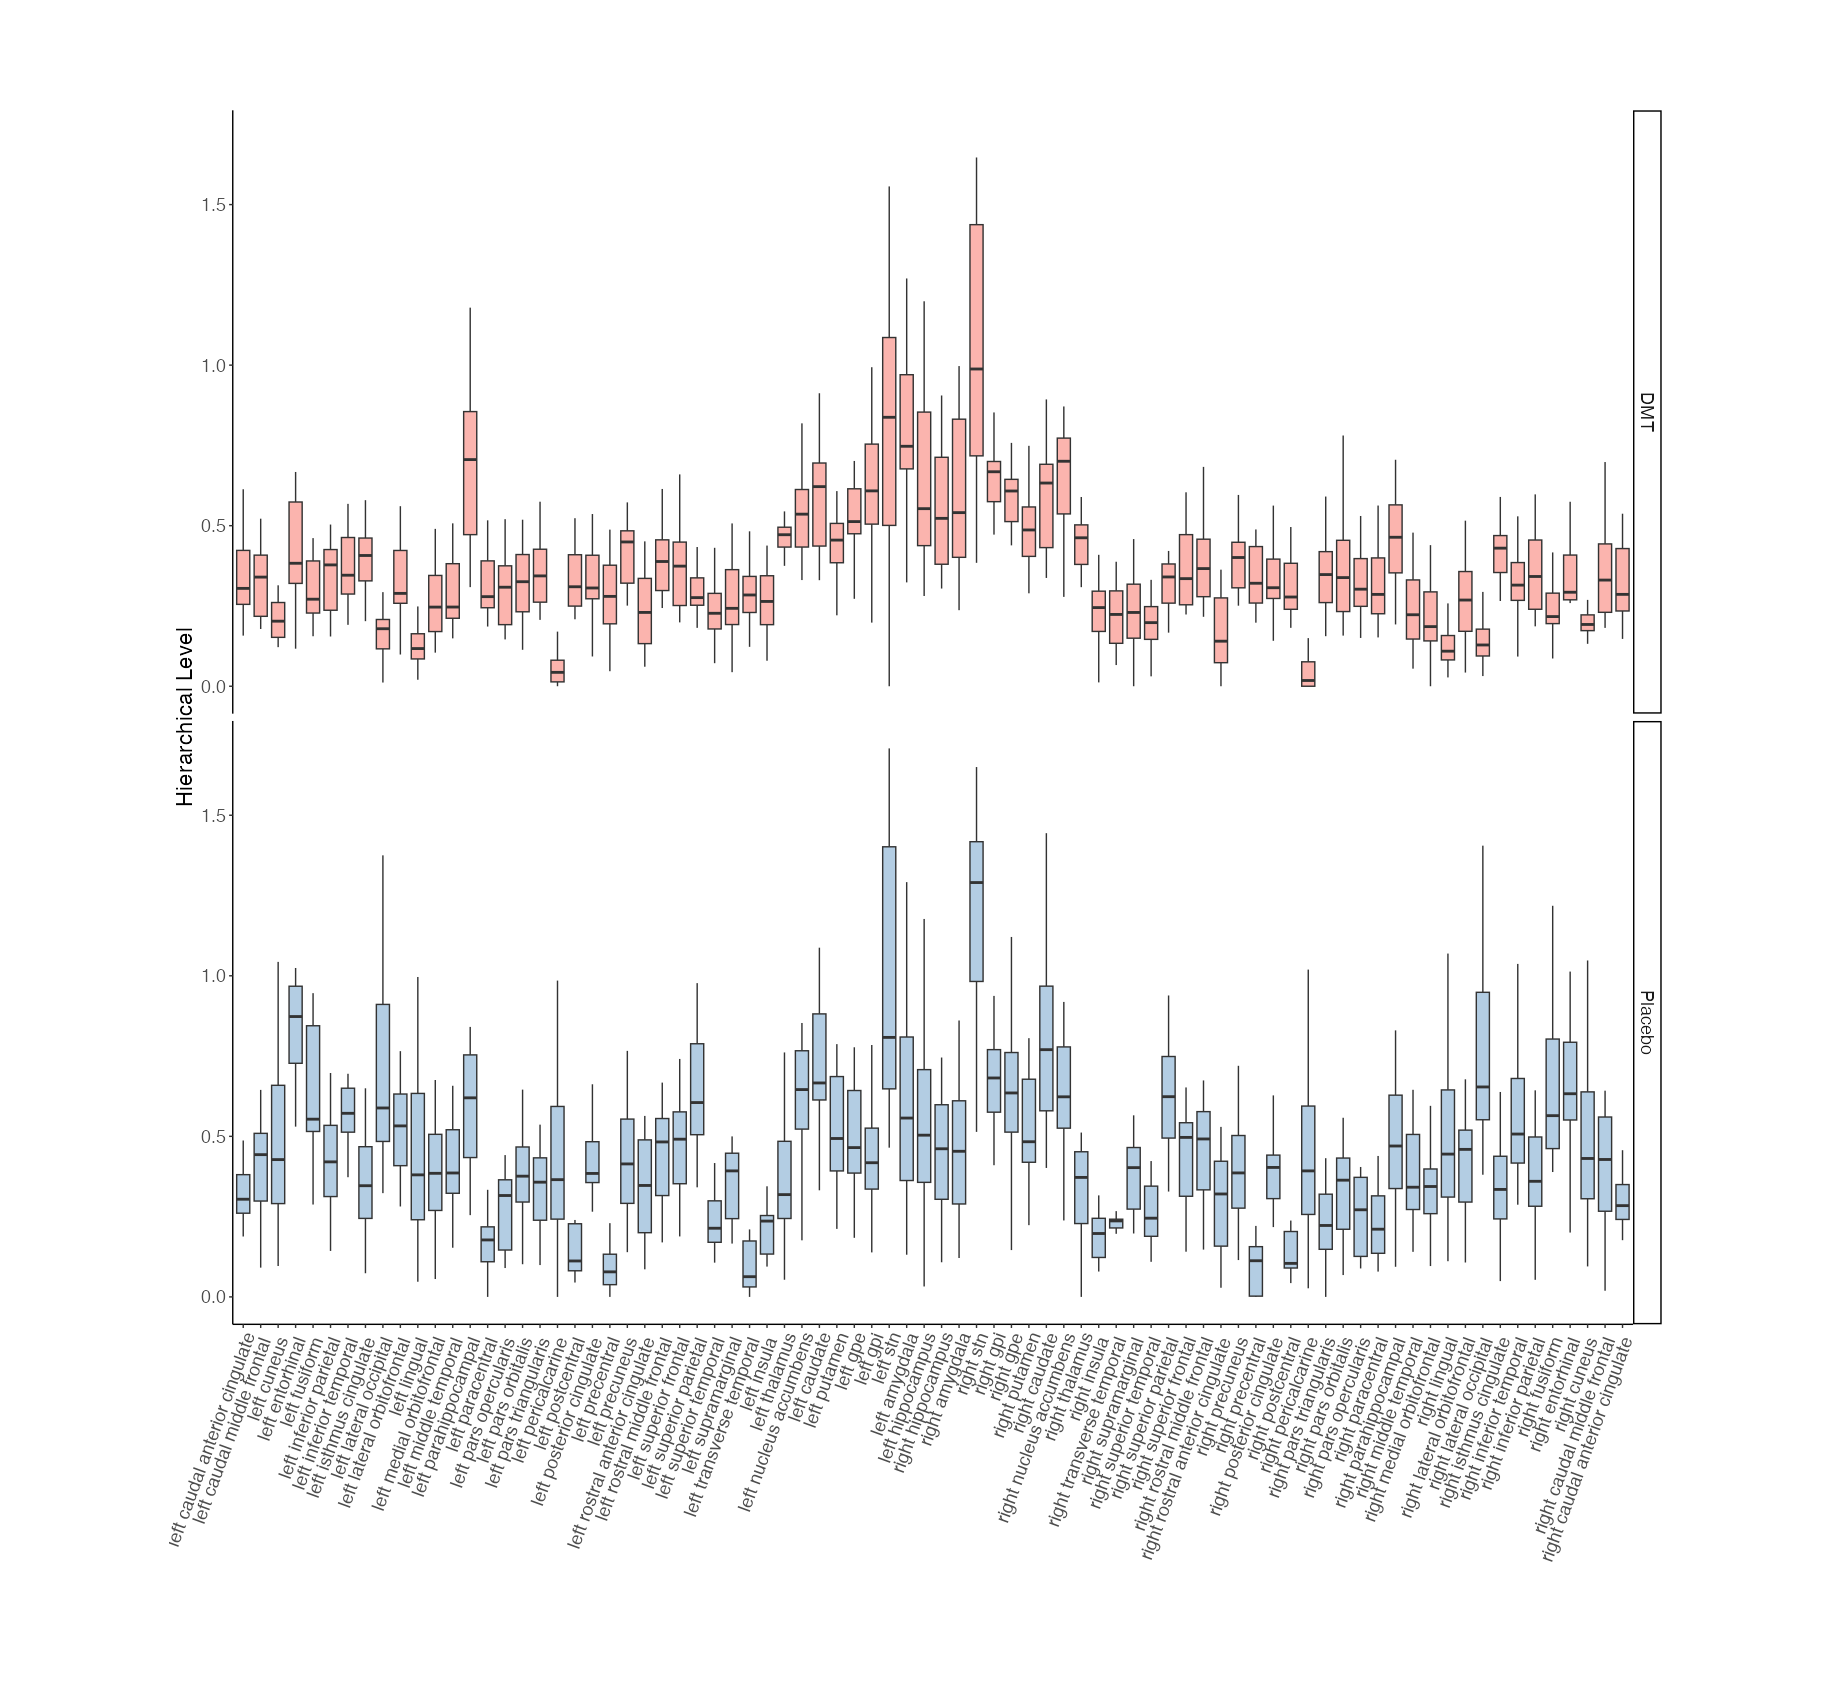
\includegraphics[width=\textwidth]{images/Appendix_ DMT HL.png}
    \caption{Hierarchical levels for each region in the DBS80 across placebo and DMT conditions.}
    \label{fig:dmthl}
\end{figure}

\begin{figure}
    \centering
    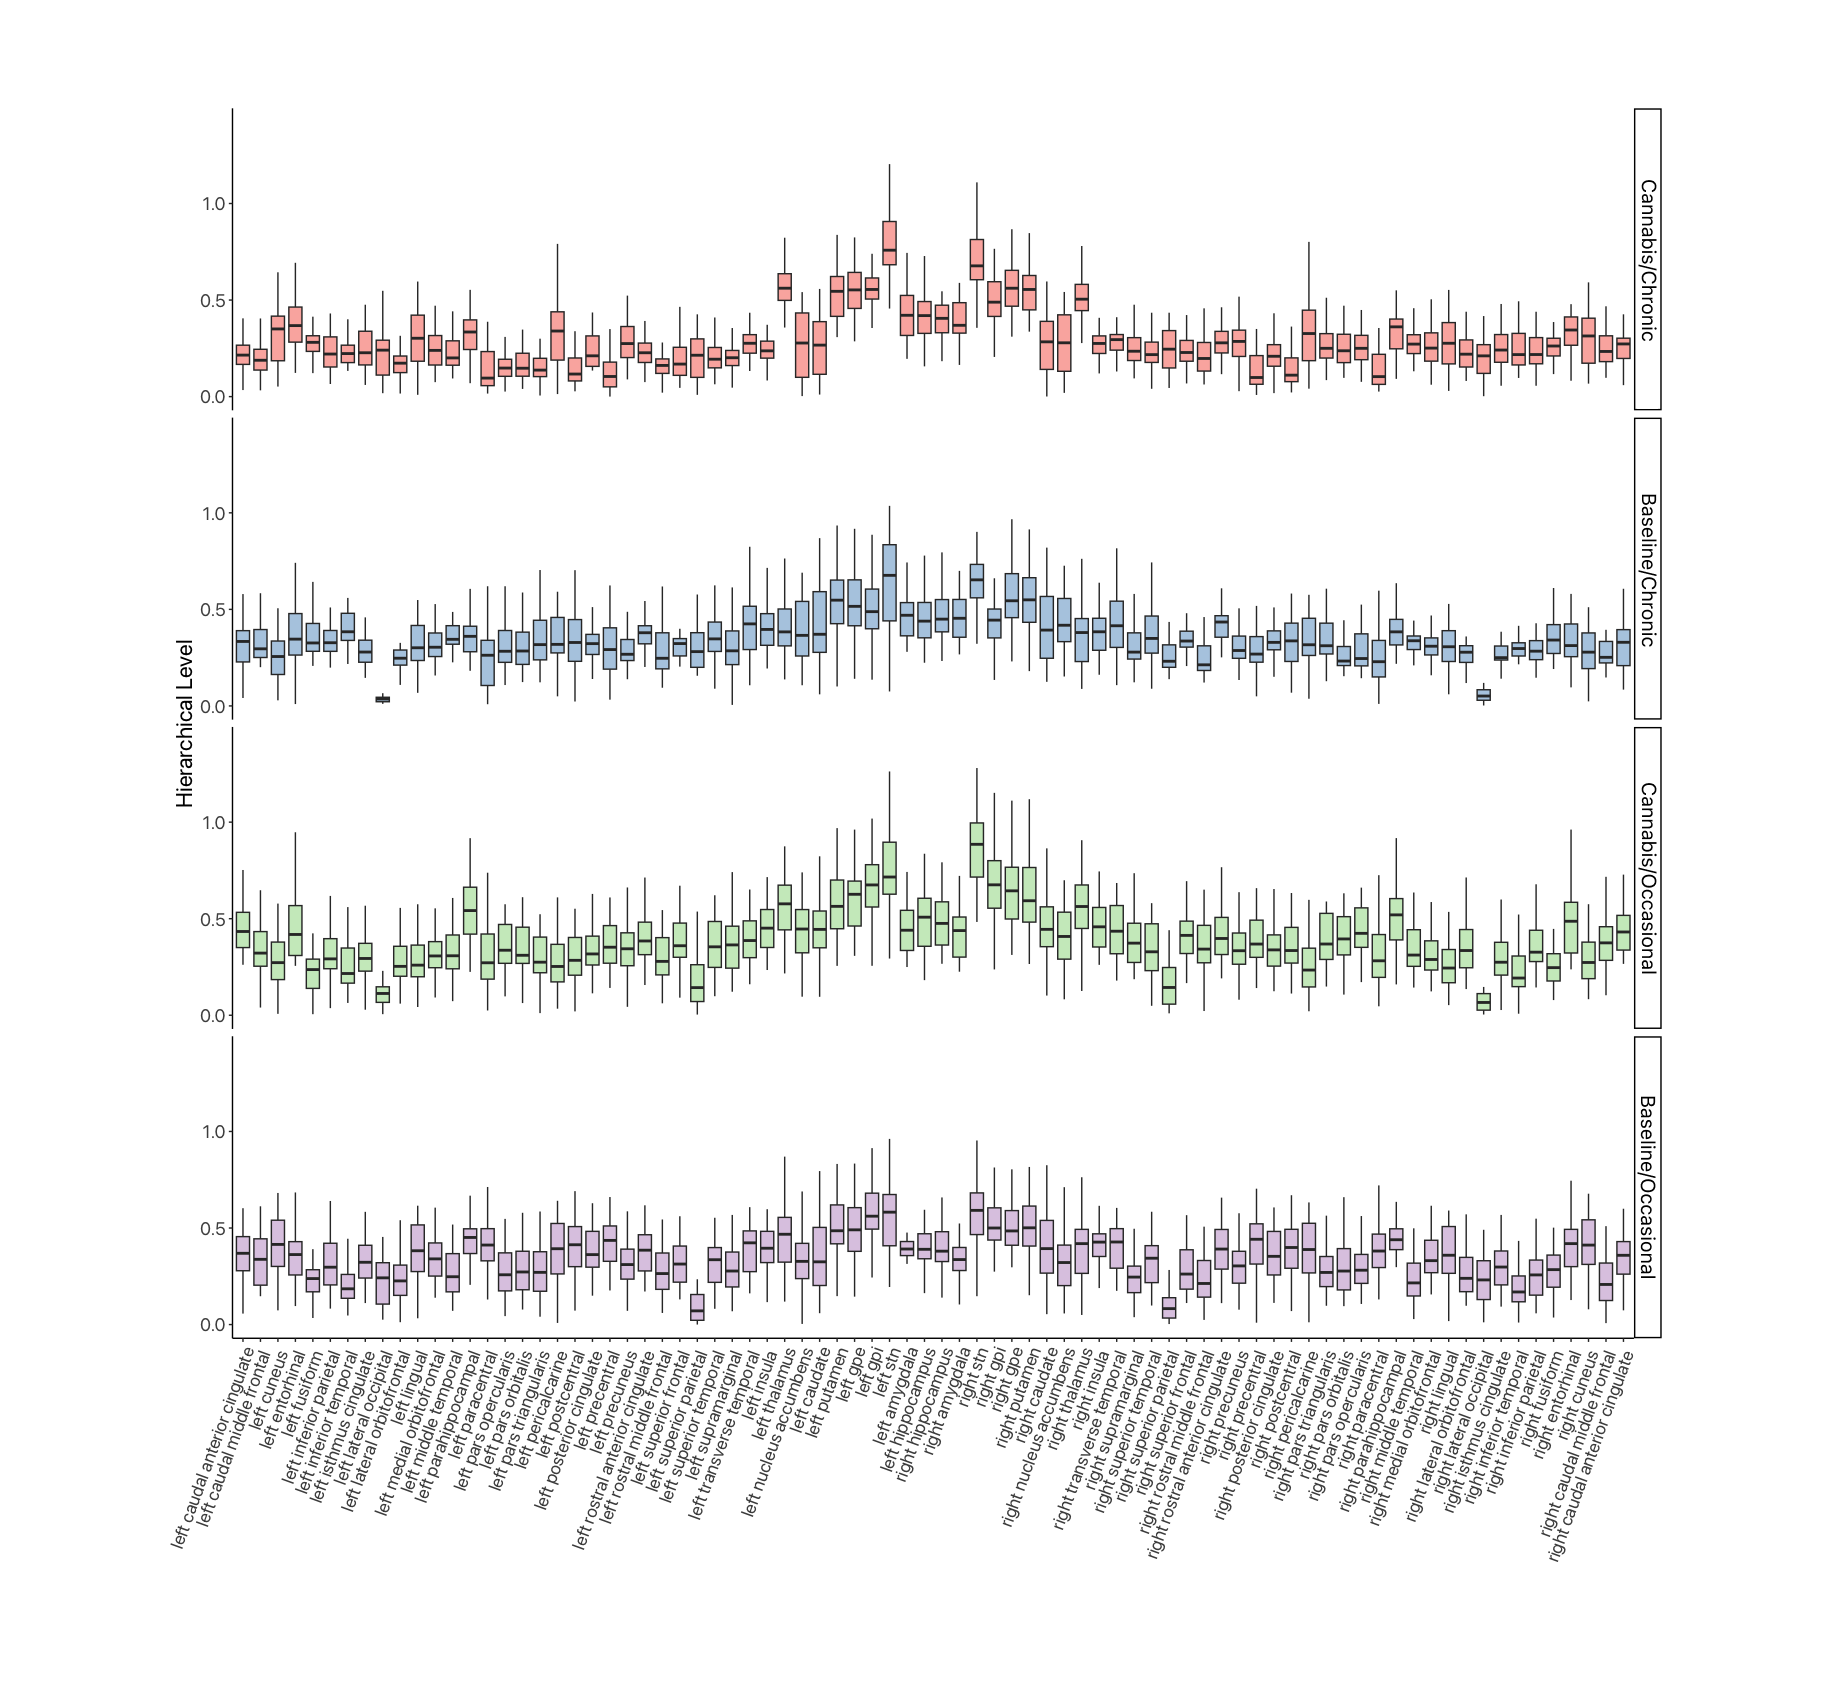
\includegraphics[width=\textwidth]{images/Appendix_ Cannab HL.png}
    \caption{Hierarchical levels for each region in the DBS80 across baseline and cannabis (both chronic and occasional users).}
    \label{fig:cannabishl}
\end{figure}